% Created by tikzDevice version 0.10.1 on 2016-11-21 07:40:38
% !TEX encoding = UTF-8 Unicode
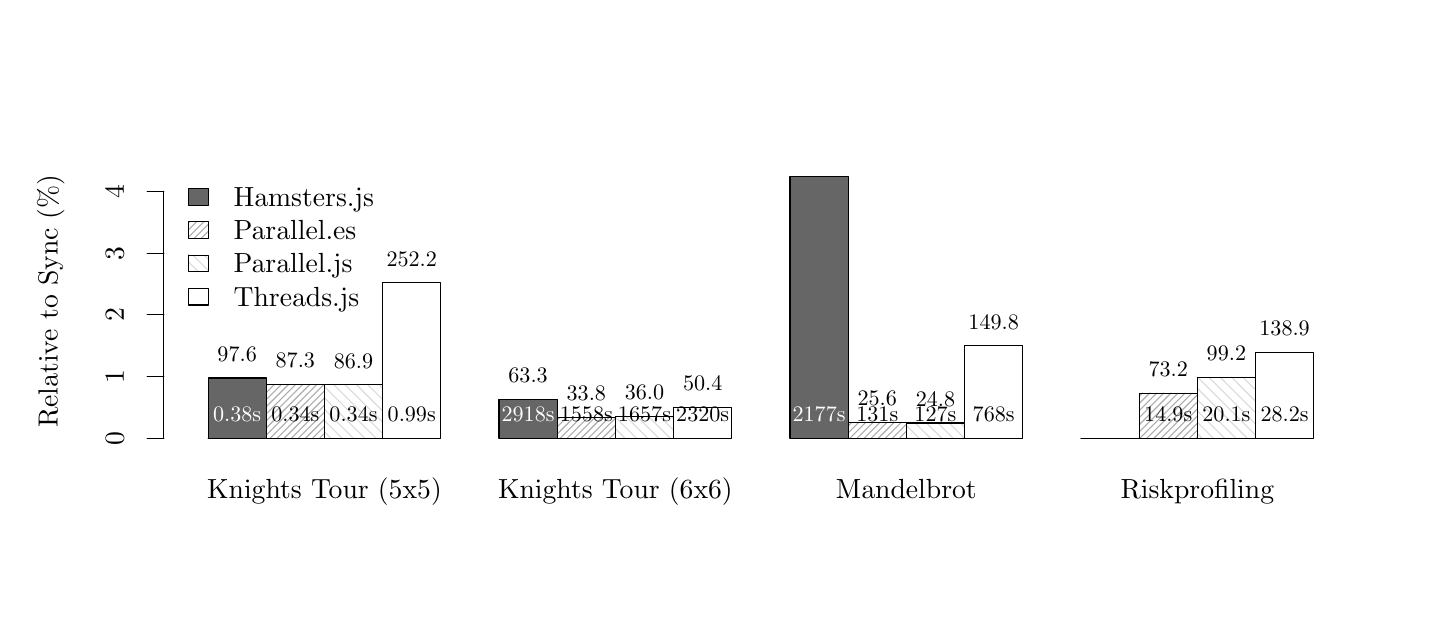
\begin{tikzpicture}[x=1pt,y=1pt]
\definecolor{fillColor}{RGB}{255,255,255}
\path[use as bounding box,fill=fillColor,fill opacity=0.00] (0,0) rectangle (505.89,209.58);
\begin{scope}
\path[clip] (  0.00,  0.00) rectangle (505.89,209.58);
\definecolor{fillColor}{gray}{0.40}

\path[fill=fillColor] ( 65.18, 61.20) --
	( 86.21, 61.20) --
	( 86.21, 82.97) --
	( 65.18, 82.97) --
	cycle;
\definecolor{drawColor}{RGB}{172,172,172}

\path[draw=drawColor,line width= 0.4pt,line join=round,line cap=round] ( 86.21, 80.26) -- ( 86.62, 80.67);

\path[draw=drawColor,line width= 0.4pt,line join=round,line cap=round] ( 86.21, 77.70) -- ( 89.18, 80.67);

\path[draw=drawColor,line width= 0.4pt,line join=round,line cap=round] ( 86.21, 75.15) -- ( 91.73, 80.67);

\path[draw=drawColor,line width= 0.4pt,line join=round,line cap=round] ( 86.21, 72.59) -- ( 94.29, 80.67);

\path[draw=drawColor,line width= 0.4pt,line join=round,line cap=round] ( 86.21, 70.04) -- ( 96.84, 80.67);

\path[draw=drawColor,line width= 0.4pt,line join=round,line cap=round] ( 86.21, 67.48) -- ( 99.40, 80.67);

\path[draw=drawColor,line width= 0.4pt,line join=round,line cap=round] ( 86.21, 64.93) -- (101.95, 80.67);

\path[draw=drawColor,line width= 0.4pt,line join=round,line cap=round] ( 86.21, 62.37) -- (104.51, 80.67);

\path[draw=drawColor,line width= 0.4pt,line join=round,line cap=round] ( 87.59, 61.20) -- (107.06, 80.67);

\path[draw=drawColor,line width= 0.4pt,line join=round,line cap=round] ( 90.15, 61.20) -- (107.24, 78.29);

\path[draw=drawColor,line width= 0.4pt,line join=round,line cap=round] ( 92.70, 61.20) -- (107.24, 75.74);

\path[draw=drawColor,line width= 0.4pt,line join=round,line cap=round] ( 95.26, 61.20) -- (107.24, 73.18);

\path[draw=drawColor,line width= 0.4pt,line join=round,line cap=round] ( 97.81, 61.20) -- (107.24, 70.63);

\path[draw=drawColor,line width= 0.4pt,line join=round,line cap=round] (100.37, 61.20) -- (107.24, 68.07);

\path[draw=drawColor,line width= 0.4pt,line join=round,line cap=round] (102.92, 61.20) -- (107.24, 65.52);

\path[draw=drawColor,line width= 0.4pt,line join=round,line cap=round] (105.48, 61.20) -- (107.24, 62.96);
\definecolor{drawColor}{RGB}{218,218,218}

\path[draw=drawColor,line width= 0.4pt,line join=round,line cap=round] (109.56, 61.20) -- (107.24, 63.53);

\path[draw=drawColor,line width= 0.4pt,line join=round,line cap=round] (113.65, 61.20) -- (107.24, 67.62);

\path[draw=drawColor,line width= 0.4pt,line join=round,line cap=round] (117.74, 61.20) -- (107.24, 71.70);

\path[draw=drawColor,line width= 0.4pt,line join=round,line cap=round] (121.83, 61.20) -- (107.24, 75.79);

\path[draw=drawColor,line width= 0.4pt,line join=round,line cap=round] (125.92, 61.20) -- (107.24, 79.88);

\path[draw=drawColor,line width= 0.4pt,line join=round,line cap=round] (128.26, 62.94) -- (110.62, 80.58);

\path[draw=drawColor,line width= 0.4pt,line join=round,line cap=round] (128.26, 67.03) -- (114.71, 80.58);

\path[draw=drawColor,line width= 0.4pt,line join=round,line cap=round] (128.26, 71.12) -- (118.80, 80.58);

\path[draw=drawColor,line width= 0.4pt,line join=round,line cap=round] (128.26, 75.21) -- (122.89, 80.58);

\path[draw=drawColor,line width= 0.4pt,line join=round,line cap=round] (128.26, 79.29) -- (126.97, 80.58);

\path[fill=fillColor] (170.32, 61.20) --
	(191.35, 61.20) --
	(191.35, 75.33) --
	(170.32, 75.33) --
	cycle;
\definecolor{drawColor}{RGB}{172,172,172}

\path[draw=drawColor,line width= 0.4pt,line join=round,line cap=round] (191.35, 67.86) -- (192.23, 68.74);

\path[draw=drawColor,line width= 0.4pt,line join=round,line cap=round] (191.35, 65.31) -- (194.78, 68.74);

\path[draw=drawColor,line width= 0.4pt,line join=round,line cap=round] (191.35, 62.75) -- (197.34, 68.74);

\path[draw=drawColor,line width= 0.4pt,line join=round,line cap=round] (192.35, 61.20) -- (199.89, 68.74);

\path[draw=drawColor,line width= 0.4pt,line join=round,line cap=round] (194.91, 61.20) -- (202.45, 68.74);

\path[draw=drawColor,line width= 0.4pt,line join=round,line cap=round] (197.46, 61.20) -- (205.00, 68.74);

\path[draw=drawColor,line width= 0.4pt,line join=round,line cap=round] (200.02, 61.20) -- (207.56, 68.74);

\path[draw=drawColor,line width= 0.4pt,line join=round,line cap=round] (202.57, 61.20) -- (210.11, 68.74);

\path[draw=drawColor,line width= 0.4pt,line join=round,line cap=round] (205.13, 61.20) -- (212.38, 68.45);

\path[draw=drawColor,line width= 0.4pt,line join=round,line cap=round] (207.68, 61.20) -- (212.38, 65.89);

\path[draw=drawColor,line width= 0.4pt,line join=round,line cap=round] (210.24, 61.20) -- (212.38, 63.34);
\definecolor{drawColor}{RGB}{218,218,218}

\path[draw=drawColor,line width= 0.4pt,line join=round,line cap=round] (215.86, 61.20) -- (212.38, 64.68);

\path[draw=drawColor,line width= 0.4pt,line join=round,line cap=round] (219.95, 61.20) -- (212.38, 68.77);

\path[draw=drawColor,line width= 0.4pt,line join=round,line cap=round] (224.03, 61.20) -- (216.01, 69.22);

\path[draw=drawColor,line width= 0.4pt,line join=round,line cap=round] (228.12, 61.20) -- (220.10, 69.22);

\path[draw=drawColor,line width= 0.4pt,line join=round,line cap=round] (232.21, 61.20) -- (224.19, 69.22);

\path[draw=drawColor,line width= 0.4pt,line join=round,line cap=round] (233.40, 64.10) -- (228.28, 69.22);

\path[draw=drawColor,line width= 0.4pt,line join=round,line cap=round] (233.40, 68.18) -- (232.36, 69.22);

\path[fill=fillColor] (275.46, 61.20) --
	(296.49, 61.20) --
	(296.49,155.92) --
	(275.46,155.92) --
	cycle;
\definecolor{drawColor}{RGB}{172,172,172}

\path[draw=drawColor,line width= 0.4pt,line join=round,line cap=round] (296.49, 65.69) -- (297.71, 66.91);

\path[draw=drawColor,line width= 0.4pt,line join=round,line cap=round] (296.49, 63.13) -- (300.26, 66.91);

\path[draw=drawColor,line width= 0.4pt,line join=round,line cap=round] (297.11, 61.20) -- (302.82, 66.91);

\path[draw=drawColor,line width= 0.4pt,line join=round,line cap=round] (299.67, 61.20) -- (305.38, 66.91);

\path[draw=drawColor,line width= 0.4pt,line join=round,line cap=round] (302.22, 61.20) -- (307.93, 66.91);

\path[draw=drawColor,line width= 0.4pt,line join=round,line cap=round] (304.78, 61.20) -- (310.49, 66.91);

\path[draw=drawColor,line width= 0.4pt,line join=round,line cap=round] (307.33, 61.20) -- (313.04, 66.91);

\path[draw=drawColor,line width= 0.4pt,line join=round,line cap=round] (309.89, 61.20) -- (315.60, 66.91);

\path[draw=drawColor,line width= 0.4pt,line join=round,line cap=round] (312.44, 61.20) -- (317.51, 66.27);

\path[draw=drawColor,line width= 0.4pt,line join=round,line cap=round] (315.00, 61.20) -- (317.51, 63.72);
\definecolor{drawColor}{RGB}{218,218,218}

\path[draw=drawColor,line width= 0.4pt,line join=round,line cap=round] (318.06, 61.20) -- (317.51, 61.75);

\path[draw=drawColor,line width= 0.4pt,line join=round,line cap=round] (322.15, 61.20) -- (317.51, 65.84);

\path[draw=drawColor,line width= 0.4pt,line join=round,line cap=round] (326.24, 61.20) -- (320.71, 66.72);

\path[draw=drawColor,line width= 0.4pt,line join=round,line cap=round] (330.33, 61.20) -- (324.80, 66.72);

\path[draw=drawColor,line width= 0.4pt,line join=round,line cap=round] (334.42, 61.20) -- (328.89, 66.72);

\path[draw=drawColor,line width= 0.4pt,line join=round,line cap=round] (338.50, 61.20) -- (332.98, 66.72);

\path[draw=drawColor,line width= 0.4pt,line join=round,line cap=round] (338.54, 65.25) -- (337.07, 66.72);

\path[fill=fillColor] (380.60, 61.20) --
	(401.63, 61.20) --
	cycle;
\definecolor{drawColor}{RGB}{172,172,172}

\path[draw=drawColor,line width= 0.4pt,line join=round,line cap=round] (401.63, 76.28) -- (402.87, 77.53);

\path[draw=drawColor,line width= 0.4pt,line join=round,line cap=round] (401.63, 73.73) -- (405.42, 77.53);

\path[draw=drawColor,line width= 0.4pt,line join=round,line cap=round] (401.63, 71.17) -- (407.98, 77.53);

\path[draw=drawColor,line width= 0.4pt,line join=round,line cap=round] (401.63, 68.62) -- (410.53, 77.53);

\path[draw=drawColor,line width= 0.4pt,line join=round,line cap=round] (401.63, 66.06) -- (413.09, 77.53);

\path[draw=drawColor,line width= 0.4pt,line join=round,line cap=round] (401.63, 63.51) -- (415.64, 77.53);

\path[draw=drawColor,line width= 0.4pt,line join=round,line cap=round] (401.87, 61.20) -- (418.20, 77.53);

\path[draw=drawColor,line width= 0.4pt,line join=round,line cap=round] (404.43, 61.20) -- (420.75, 77.53);

\path[draw=drawColor,line width= 0.4pt,line join=round,line cap=round] (406.98, 61.20) -- (422.65, 76.87);

\path[draw=drawColor,line width= 0.4pt,line join=round,line cap=round] (409.54, 61.20) -- (422.65, 74.32);

\path[draw=drawColor,line width= 0.4pt,line join=round,line cap=round] (412.09, 61.20) -- (422.65, 71.76);

\path[draw=drawColor,line width= 0.4pt,line join=round,line cap=round] (414.65, 61.20) -- (422.65, 69.21);

\path[draw=drawColor,line width= 0.4pt,line join=round,line cap=round] (417.20, 61.20) -- (422.65, 66.65);

\path[draw=drawColor,line width= 0.4pt,line join=round,line cap=round] (419.76, 61.20) -- (422.65, 64.10);

\path[draw=drawColor,line width= 0.4pt,line join=round,line cap=round] (422.31, 61.20) -- (422.65, 61.54);
\definecolor{drawColor}{RGB}{218,218,218}

\path[draw=drawColor,line width= 0.4pt,line join=round,line cap=round] (424.36, 61.20) -- (422.65, 62.90);

\path[draw=drawColor,line width= 0.4pt,line join=round,line cap=round] (428.44, 61.20) -- (422.65, 66.99);

\path[draw=drawColor,line width= 0.4pt,line join=round,line cap=round] (432.53, 61.20) -- (422.65, 71.08);

\path[draw=drawColor,line width= 0.4pt,line join=round,line cap=round] (436.62, 61.20) -- (422.65, 75.17);

\path[draw=drawColor,line width= 0.4pt,line join=round,line cap=round] (440.71, 61.20) -- (422.65, 79.26);

\path[draw=drawColor,line width= 0.4pt,line join=round,line cap=round] (443.68, 62.32) -- (422.68, 83.32);

\path[draw=drawColor,line width= 0.4pt,line join=round,line cap=round] (443.68, 66.40) -- (426.77, 83.32);

\path[draw=drawColor,line width= 0.4pt,line join=round,line cap=round] (443.68, 70.49) -- (430.86, 83.32);

\path[draw=drawColor,line width= 0.4pt,line join=round,line cap=round] (443.68, 74.58) -- (434.95, 83.32);

\path[draw=drawColor,line width= 0.4pt,line join=round,line cap=round] (443.68, 78.67) -- (439.03, 83.32);

\path[draw=drawColor,line width= 0.4pt,line join=round,line cap=round] (443.68, 82.76) -- (443.12, 83.32);
\definecolor{drawColor}{RGB}{0,0,0}

\path[draw=drawColor,line width= 0.4pt,line join=round,line cap=round] ( 65.18, 61.20) --
	( 86.21, 61.20) --
	( 86.21, 82.97) --
	( 65.18, 82.97) --
	( 65.18, 61.20);

\path[draw=drawColor,line width= 0.4pt,line join=round,line cap=round] ( 86.21, 61.20) --
	(107.24, 61.20) --
	(107.24, 80.67) --
	( 86.21, 80.67) --
	( 86.21, 61.20);

\path[draw=drawColor,line width= 0.4pt,line join=round,line cap=round] (107.24, 61.20) --
	(128.26, 61.20) --
	(128.26, 80.58) --
	(107.24, 80.58) --
	(107.24, 61.20);

\path[draw=drawColor,line width= 0.4pt,line join=round,line cap=round] (128.26, 61.20) --
	(149.29, 61.20) --
	(149.29,117.45) --
	(128.26,117.45) --
	(128.26, 61.20);

\path[draw=drawColor,line width= 0.4pt,line join=round,line cap=round] (170.32, 61.20) --
	(191.35, 61.20) --
	(191.35, 75.33) --
	(170.32, 75.33) --
	(170.32, 61.20);

\path[draw=drawColor,line width= 0.4pt,line join=round,line cap=round] (191.35, 61.20) --
	(212.38, 61.20) --
	(212.38, 68.74) --
	(191.35, 68.74) --
	(191.35, 61.20);

\path[draw=drawColor,line width= 0.4pt,line join=round,line cap=round] (212.38, 61.20) --
	(233.40, 61.20) --
	(233.40, 69.22) --
	(212.38, 69.22) --
	(212.38, 61.20);

\path[draw=drawColor,line width= 0.4pt,line join=round,line cap=round] (233.40, 61.20) --
	(254.43, 61.20) --
	(254.43, 72.43) --
	(233.40, 72.43) --
	(233.40, 61.20);

\path[draw=drawColor,line width= 0.4pt,line join=round,line cap=round] (275.46, 61.20) --
	(296.49, 61.20) --
	(296.49,155.92) --
	(275.46,155.92) --
	(275.46, 61.20);

\path[draw=drawColor,line width= 0.4pt,line join=round,line cap=round] (296.49, 61.20) --
	(317.51, 61.20) --
	(317.51, 66.91) --
	(296.49, 66.91) --
	(296.49, 61.20);

\path[draw=drawColor,line width= 0.4pt,line join=round,line cap=round] (317.51, 61.20) --
	(338.54, 61.20) --
	(338.54, 66.72) --
	(317.51, 66.72) --
	(317.51, 61.20);

\path[draw=drawColor,line width= 0.4pt,line join=round,line cap=round] (338.54, 61.20) --
	(359.57, 61.20) --
	(359.57, 94.61) --
	(338.54, 94.61) --
	(338.54, 61.20);

\path[draw=drawColor,line width= 0.4pt,line join=round,line cap=round] (380.60, 61.20) --
	(401.63, 61.20) --
	(380.60, 61.20);

\path[draw=drawColor,line width= 0.4pt,line join=round,line cap=round] (401.63, 61.20) --
	(422.65, 61.20) --
	(422.65, 77.53) --
	(401.63, 77.53) --
	(401.63, 61.20);

\path[draw=drawColor,line width= 0.4pt,line join=round,line cap=round] (422.65, 61.20) --
	(443.68, 61.20) --
	(443.68, 83.32) --
	(422.65, 83.32) --
	(422.65, 61.20);

\path[draw=drawColor,line width= 0.4pt,line join=round,line cap=round] (443.68, 61.20) --
	(464.71, 61.20) --
	(464.71, 92.19) --
	(443.68, 92.19) --
	(443.68, 61.20);
\end{scope}
\begin{scope}
\path[clip] (  0.00,  0.00) rectangle (505.89,209.58);
\definecolor{drawColor}{RGB}{0,0,0}

\node[text=drawColor,anchor=base,inner sep=0pt, outer sep=0pt, scale=  1.00] at (107.24, 39.60) {Knights Tour (5x5)};

\node[text=drawColor,anchor=base,inner sep=0pt, outer sep=0pt, scale=  1.00] at (212.38, 39.60) {Knights Tour (6x6)};

\node[text=drawColor,anchor=base,inner sep=0pt, outer sep=0pt, scale=  1.00] at (317.51, 39.60) {Mandelbrot};

\node[text=drawColor,anchor=base,inner sep=0pt, outer sep=0pt, scale=  1.00] at (422.65, 39.60) {Riskprofiling};
\end{scope}
\begin{scope}
\path[clip] (  0.00,  0.00) rectangle (505.89,209.58);
\definecolor{drawColor}{RGB}{0,0,0}

\node[text=drawColor,rotate= 90.00,anchor=base,inner sep=0pt, outer sep=0pt, scale=  1.00] at ( 10.80,110.79) {Relative to Sync ({\%})};
\end{scope}
\begin{scope}
\path[clip] (  0.00,  0.00) rectangle (505.89,209.58);
\definecolor{drawColor}{RGB}{0,0,0}

\path[draw=drawColor,line width= 0.4pt,line join=round,line cap=round] ( 49.20, 61.20) -- ( 49.20,150.41);

\path[draw=drawColor,line width= 0.4pt,line join=round,line cap=round] ( 49.20, 61.20) -- ( 43.20, 61.20);

\path[draw=drawColor,line width= 0.4pt,line join=round,line cap=round] ( 49.20, 83.50) -- ( 43.20, 83.50);

\path[draw=drawColor,line width= 0.4pt,line join=round,line cap=round] ( 49.20,105.81) -- ( 43.20,105.81);

\path[draw=drawColor,line width= 0.4pt,line join=round,line cap=round] ( 49.20,128.11) -- ( 43.20,128.11);

\path[draw=drawColor,line width= 0.4pt,line join=round,line cap=round] ( 49.20,150.41) -- ( 43.20,150.41);

\node[text=drawColor,rotate= 90.00,anchor=base,inner sep=0pt, outer sep=0pt, scale=  1.00] at ( 34.80, 61.20) {0};

\node[text=drawColor,rotate= 90.00,anchor=base,inner sep=0pt, outer sep=0pt, scale=  1.00] at ( 34.80, 83.50) {1};

\node[text=drawColor,rotate= 90.00,anchor=base,inner sep=0pt, outer sep=0pt, scale=  1.00] at ( 34.80,105.81) {2};

\node[text=drawColor,rotate= 90.00,anchor=base,inner sep=0pt, outer sep=0pt, scale=  1.00] at ( 34.80,128.11) {3};

\node[text=drawColor,rotate= 90.00,anchor=base,inner sep=0pt, outer sep=0pt, scale=  1.00] at ( 34.80,150.41) {4};
\end{scope}
\begin{scope}
\path[clip] ( 49.20, 61.20) rectangle (480.69,160.38);
\definecolor{fillColor}{gray}{0.40}

\path[fill=fillColor] ( 58.20,151.38) --
	( 65.40,151.38) --
	( 65.40,145.38) --
	( 58.20,145.38) --
	cycle;
\definecolor{drawColor}{RGB}{172,172,172}

\path[draw=drawColor,line width= 0.4pt,line join=round,line cap=round] ( 58.20,139.12) -- ( 58.46,139.38);

\path[draw=drawColor,line width= 0.4pt,line join=round,line cap=round] ( 58.20,136.57) -- ( 61.01,139.38);

\path[draw=drawColor,line width= 0.4pt,line join=round,line cap=round] ( 58.20,134.01) -- ( 63.57,139.38);

\path[draw=drawColor,line width= 0.4pt,line join=round,line cap=round] ( 60.12,133.38) -- ( 65.40,138.66);

\path[draw=drawColor,line width= 0.4pt,line join=round,line cap=round] ( 62.68,133.38) -- ( 65.40,136.10);

\path[draw=drawColor,line width= 0.4pt,line join=round,line cap=round] ( 65.23,133.38) -- ( 65.40,133.55);
\definecolor{drawColor}{RGB}{218,218,218}

\path[draw=drawColor,line width= 0.4pt,line join=round,line cap=round] ( 61.65,121.38) -- ( 58.20,124.83);

\path[draw=drawColor,line width= 0.4pt,line join=round,line cap=round] ( 65.40,121.72) -- ( 59.73,127.38);

\path[draw=drawColor,line width= 0.4pt,line join=round,line cap=round] ( 65.40,125.81) -- ( 63.82,127.38);
\definecolor{drawColor}{RGB}{0,0,0}

\path[draw=drawColor,line width= 0.4pt,line join=round,line cap=round] ( 58.20,151.38) --
	( 65.40,151.38) --
	( 65.40,145.38) --
	( 58.20,145.38) --
	( 58.20,151.38);

\path[draw=drawColor,line width= 0.4pt,line join=round,line cap=round] ( 58.20,139.38) --
	( 65.40,139.38) --
	( 65.40,133.38) --
	( 58.20,133.38) --
	( 58.20,139.38);

\path[draw=drawColor,line width= 0.4pt,line join=round,line cap=round] ( 58.20,127.38) --
	( 65.40,127.38) --
	( 65.40,121.38) --
	( 58.20,121.38) --
	( 58.20,127.38);

\path[draw=drawColor,line width= 0.4pt,line join=round,line cap=round] ( 58.20,115.38) --
	( 65.40,115.38) --
	( 65.40,109.38) --
	( 58.20,109.38) --
	( 58.20,115.38);

\node[text=drawColor,anchor=base west,inner sep=0pt, outer sep=0pt, scale=  1.00] at ( 74.40,144.94) {Hamsters.js};

\node[text=drawColor,anchor=base west,inner sep=0pt, outer sep=0pt, scale=  1.00] at ( 74.40,132.94) {Parallel.es};

\node[text=drawColor,anchor=base west,inner sep=0pt, outer sep=0pt, scale=  1.00] at ( 74.40,120.94) {Parallel.js};

\node[text=drawColor,anchor=base west,inner sep=0pt, outer sep=0pt, scale=  1.00] at ( 74.40,108.94) {Threads.js};

\node[text=drawColor,anchor=base,inner sep=0pt, outer sep=0pt, scale=  0.80] at ( 75.70, 88.97) {97.6};

\node[text=drawColor,anchor=base,inner sep=0pt, outer sep=0pt, scale=  0.80] at ( 96.72, 86.67) {87.3};

\node[text=drawColor,anchor=base,inner sep=0pt, outer sep=0pt, scale=  0.80] at (117.75, 86.58) {86.9};

\node[text=drawColor,anchor=base,inner sep=0pt, outer sep=0pt, scale=  0.80] at (138.78,123.45) {252.2};

\node[text=drawColor,anchor=base,inner sep=0pt, outer sep=0pt, scale=  0.80] at (180.83, 81.33) {63.3};

\node[text=drawColor,anchor=base,inner sep=0pt, outer sep=0pt, scale=  0.80] at (201.86, 74.74) {33.8};

\node[text=drawColor,anchor=base,inner sep=0pt, outer sep=0pt, scale=  0.80] at (222.89, 75.22) {36.0};

\node[text=drawColor,anchor=base,inner sep=0pt, outer sep=0pt, scale=  0.80] at (243.92, 78.43) {50.4};

\node[text=drawColor,anchor=base,inner sep=0pt, outer sep=0pt, scale=  0.80] at (285.97,161.92) {424.7};

\node[text=drawColor,anchor=base,inner sep=0pt, outer sep=0pt, scale=  0.80] at (307.00, 72.91) {25.6};

\node[text=drawColor,anchor=base,inner sep=0pt, outer sep=0pt, scale=  0.80] at (328.03, 72.72) {24.8};

\node[text=drawColor,anchor=base,inner sep=0pt, outer sep=0pt, scale=  0.80] at (349.06,100.61) {149.8};

\node[text=drawColor,anchor=base,inner sep=0pt, outer sep=0pt, scale=  0.80] at (412.14, 83.53) {73.2};

\node[text=drawColor,anchor=base,inner sep=0pt, outer sep=0pt, scale=  0.80] at (433.17, 89.32) {99.2};

\node[text=drawColor,anchor=base,inner sep=0pt, outer sep=0pt, scale=  0.80] at (454.19, 98.19) {138.9};
\definecolor{drawColor}{RGB}{255,255,255}

\node[text=drawColor,anchor=base,inner sep=0pt, outer sep=0pt, scale=  0.80] at ( 75.70, 67.20) {0.38s};
\definecolor{drawColor}{RGB}{0,0,0}

\node[text=drawColor,anchor=base,inner sep=0pt, outer sep=0pt, scale=  0.80] at ( 96.72, 67.20) {0.34s};

\node[text=drawColor,anchor=base,inner sep=0pt, outer sep=0pt, scale=  0.80] at (117.75, 67.20) {0.34s};

\node[text=drawColor,anchor=base,inner sep=0pt, outer sep=0pt, scale=  0.80] at (138.78, 67.20) {0.99s};
\definecolor{drawColor}{RGB}{255,255,255}

\node[text=drawColor,anchor=base,inner sep=0pt, outer sep=0pt, scale=  0.80] at (180.83, 67.20) {2918s};
\definecolor{drawColor}{RGB}{0,0,0}

\node[text=drawColor,anchor=base,inner sep=0pt, outer sep=0pt, scale=  0.80] at (201.86, 67.20) {1558s};

\node[text=drawColor,anchor=base,inner sep=0pt, outer sep=0pt, scale=  0.80] at (222.89, 67.20) {1657s};

\node[text=drawColor,anchor=base,inner sep=0pt, outer sep=0pt, scale=  0.80] at (243.92, 67.20) {2320s};
\definecolor{drawColor}{RGB}{255,255,255}

\node[text=drawColor,anchor=base,inner sep=0pt, outer sep=0pt, scale=  0.80] at (285.97, 67.20) {2177s};
\definecolor{drawColor}{RGB}{0,0,0}

\node[text=drawColor,anchor=base,inner sep=0pt, outer sep=0pt, scale=  0.80] at (307.00, 67.20) {131s};

\node[text=drawColor,anchor=base,inner sep=0pt, outer sep=0pt, scale=  0.80] at (328.03, 67.20) {127s};

\node[text=drawColor,anchor=base,inner sep=0pt, outer sep=0pt, scale=  0.80] at (349.06, 67.20) {768s};

\node[text=drawColor,anchor=base,inner sep=0pt, outer sep=0pt, scale=  0.80] at (412.14, 67.20) {14.9s};

\node[text=drawColor,anchor=base,inner sep=0pt, outer sep=0pt, scale=  0.80] at (433.17, 67.20) {20.1s};

\node[text=drawColor,anchor=base,inner sep=0pt, outer sep=0pt, scale=  0.80] at (454.19, 67.20) {28.2s};
\end{scope}
\end{tikzpicture}
